\chapter{Work Plan}
\lhead{\emph{Work Plan}}

\begin{figure}[h!]
  \centering
  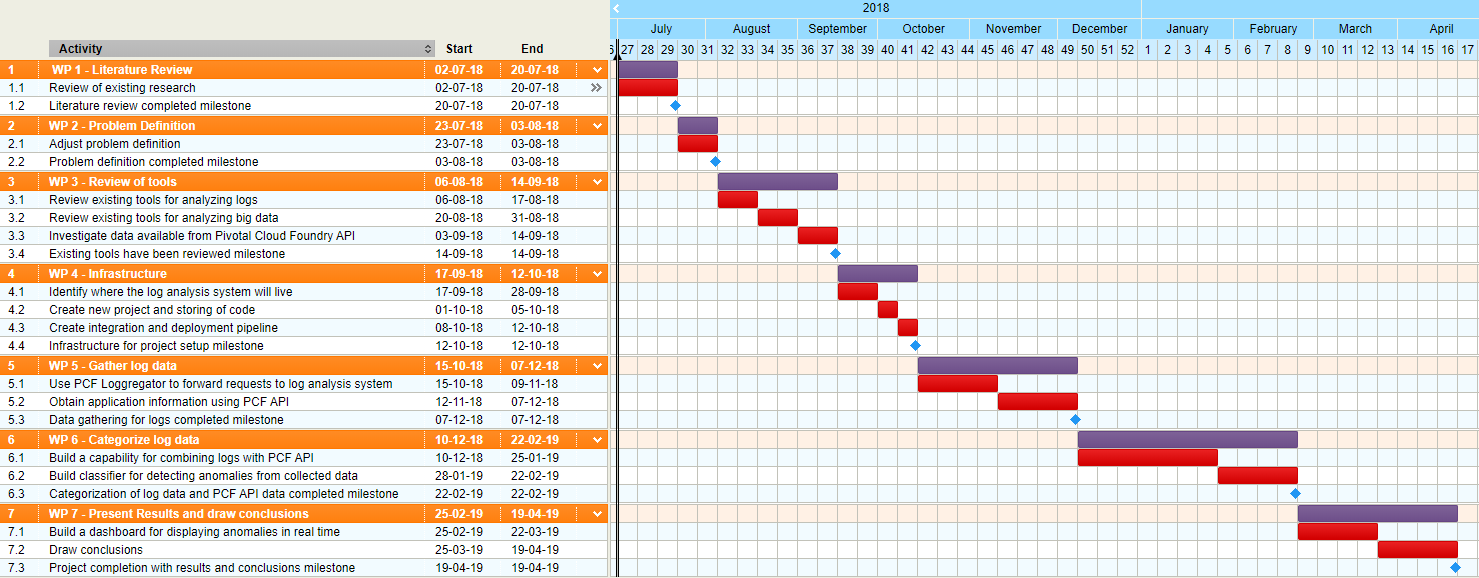
\includegraphics[width=1.0\textwidth]{./figures/gantt.png}
  \caption{gantt}
  \label{fig:gantt}
\end{figure}

\begin{itemize}
  \item \textbf{WP 1} Literature review - 3 weeks - In this work package I will perform a literature review on existing approaches to log analysis.
  \item \textbf{WP 2} Problem definition - 2 weeks - Based on the literature review, the challenges of log analysis will be evaluated further. The challenges will produce the definition of key research questions.
  \item \textbf{WP 3} Review of tools - 6 weeks - In this work package I will be looking at the available tools available for log analysis. I will also be looking at data available in the Cloud Foundry API.
  \item \textbf{WP 4} Infrastructure - 4 weeks - This work package involves setting up the infrastructure for my project. I will be looking at solutions for storing my code and where best to run the application as well as creating a continuous integration pipeline for rapid development.
  \item \textbf{WP 5} Gather log data - 8 weeks - In this work package I will be sourcing logs that will be used for comparative analysis of my service. I will also be setting up Cloud Foundries loggregator to forward all logs to the analysis service.
  \item \textbf{WP 6} Categorize log data - 11 weeks - In this work package I will deliver the necessary log analysis algorithms to correctly identify root causes of failures. I will also compare log analysis only results with log analysis plus Cloud Foundry API results.
  \item \textbf{WP 7} Present Results and draw conclusions - 8 weeks - In this work package I will be assembling a dashboard to display root causes of issues to users. Once this is complete I will be preparing a report outlining the project observations and conclusions.
\end{itemize}